\let\negmedspace\undefined
\let\negthickspace\undefined
\documentclass[journal,12pt,twocolumn]{IEEEtran}
\usepackage{gensymb}
\usepackage{amssymb}
\usepackage[cmex10]{amsmath}
\usepackage{amsthm}
\usepackage[justification=centering]{caption}
\usepackage{bm}
\usepackage{longtable}
\usepackage{enumitem}
\usepackage{mathtools}
 \usepackage{tikz}
\usepackage[breaklinks=true]{hyperref}
\usepackage{listings}
\usepackage{color}                                            %%
\usepackage{array}                                            %%
\usepackage{longtable}                                        %%
\usepackage{calc}                                             %%
\usepackage{multirow}                                         %%
\usepackage{hhline}                                           %%
\usepackage{ifthen}                                           %%
\usepackage{lscape}     
\usepackage{multicol}
\newcommand{\solution}{\noindent \textbf{Solution: }}
\begin{document}
\vspace{3cm}
\title{Assignment I (ICSE Class 10 2018)}
\author{Gautam Singh (CS21BTECH11018)}
% make the title area
\maketitle
\begin{enumerate}[label=\arabic{enumi}. , start = 5]
\item
\begin{enumerate}[label=\alph{enumii}. , start = 3]
\item Use graph paper for this question (Take 2cm = 1 unit along both x and y axis). ABCD is a quadrilateral whose vertices are A(2,2), B(2,$-$2), C(0,$-$1) and D(0,1).
\begin{enumerate}[label=(\roman{enumiii})]
\item Reflect quadrilateral ABCD on the \textit{y}-axis and name it as A\textquotesingle B\textquotesingle CD.
\item Write down the coordinates of A{\textquotesingle} and B\textquotesingle .
\item Name two points which are invariant under the above reflection.
\item Name the polygon A\textquotesingle B\textquotesingle CD.
\end{enumerate}
\solution 
\begin{enumerate}[label=(\roman{enumiii})]
\item The plot of quadrilateral ABCD after reflection on the \textit{y}-axis is as shown:
\begin{figure}[h]
\centering
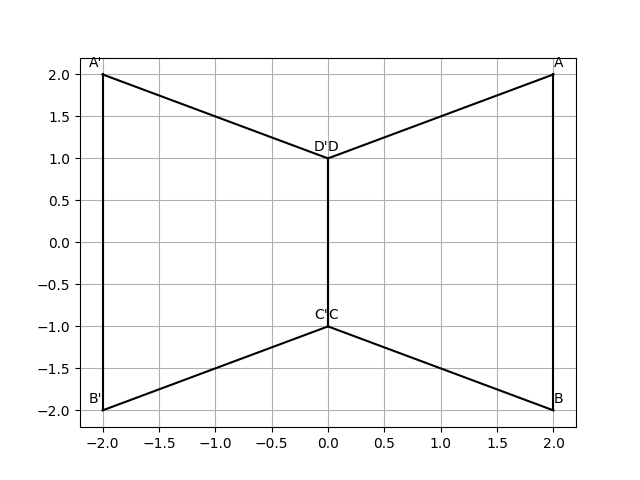
\includegraphics[scale=0.5]{./figs/5.3.1.png}
\end{figure}
\item The coordinates of A{\textquotesingle} and B{\textquotesingle} are ($-$2,2) and ($-$2,$-$2) respectively.
\item The two points which are invariant under reflection are C(0,$-$1) and D(0,1).
\item The polygon A\textquotesingle B\textquotesingle CD is an isosceles trapezium.
\end{enumerate}
\end{enumerate}
\end{enumerate}
\end{document}